\documentclass[12pt,]{article}
\usepackage{lmodern}
\usepackage{amssymb,amsmath}
\usepackage{ifxetex,ifluatex}
\usepackage{fixltx2e} % provides \textsubscript
\ifnum 0\ifxetex 1\fi\ifluatex 1\fi=0 % if pdftex
  \usepackage[T1]{fontenc}
  \usepackage[utf8]{inputenc}
\else % if luatex or xelatex
  \ifxetex
    \usepackage{mathspec}
  \else
    \usepackage{fontspec}
  \fi
  \defaultfontfeatures{Ligatures=TeX,Scale=MatchLowercase}
\fi
% use upquote if available, for straight quotes in verbatim environments
\IfFileExists{upquote.sty}{\usepackage{upquote}}{}
% use microtype if available
\IfFileExists{microtype.sty}{%
\usepackage{microtype}
\UseMicrotypeSet[protrusion]{basicmath} % disable protrusion for tt fonts
}{}
\usepackage[margin=1in]{geometry}
\usepackage{hyperref}
\hypersetup{unicode=true,
            pdftitle={STAT 6910: HW 5},
            pdfauthor={David Angeles},
            pdfborder={0 0 0},
            breaklinks=true}
\urlstyle{same}  % don't use monospace font for urls
\usepackage{color}
\usepackage{fancyvrb}
\newcommand{\VerbBar}{|}
\newcommand{\VERB}{\Verb[commandchars=\\\{\}]}
\DefineVerbatimEnvironment{Highlighting}{Verbatim}{commandchars=\\\{\}}
% Add ',fontsize=\small' for more characters per line
\usepackage{framed}
\definecolor{shadecolor}{RGB}{248,248,248}
\newenvironment{Shaded}{\begin{snugshade}}{\end{snugshade}}
\newcommand{\KeywordTok}[1]{\textcolor[rgb]{0.13,0.29,0.53}{\textbf{#1}}}
\newcommand{\DataTypeTok}[1]{\textcolor[rgb]{0.13,0.29,0.53}{#1}}
\newcommand{\DecValTok}[1]{\textcolor[rgb]{0.00,0.00,0.81}{#1}}
\newcommand{\BaseNTok}[1]{\textcolor[rgb]{0.00,0.00,0.81}{#1}}
\newcommand{\FloatTok}[1]{\textcolor[rgb]{0.00,0.00,0.81}{#1}}
\newcommand{\ConstantTok}[1]{\textcolor[rgb]{0.00,0.00,0.00}{#1}}
\newcommand{\CharTok}[1]{\textcolor[rgb]{0.31,0.60,0.02}{#1}}
\newcommand{\SpecialCharTok}[1]{\textcolor[rgb]{0.00,0.00,0.00}{#1}}
\newcommand{\StringTok}[1]{\textcolor[rgb]{0.31,0.60,0.02}{#1}}
\newcommand{\VerbatimStringTok}[1]{\textcolor[rgb]{0.31,0.60,0.02}{#1}}
\newcommand{\SpecialStringTok}[1]{\textcolor[rgb]{0.31,0.60,0.02}{#1}}
\newcommand{\ImportTok}[1]{#1}
\newcommand{\CommentTok}[1]{\textcolor[rgb]{0.56,0.35,0.01}{\textit{#1}}}
\newcommand{\DocumentationTok}[1]{\textcolor[rgb]{0.56,0.35,0.01}{\textbf{\textit{#1}}}}
\newcommand{\AnnotationTok}[1]{\textcolor[rgb]{0.56,0.35,0.01}{\textbf{\textit{#1}}}}
\newcommand{\CommentVarTok}[1]{\textcolor[rgb]{0.56,0.35,0.01}{\textbf{\textit{#1}}}}
\newcommand{\OtherTok}[1]{\textcolor[rgb]{0.56,0.35,0.01}{#1}}
\newcommand{\FunctionTok}[1]{\textcolor[rgb]{0.00,0.00,0.00}{#1}}
\newcommand{\VariableTok}[1]{\textcolor[rgb]{0.00,0.00,0.00}{#1}}
\newcommand{\ControlFlowTok}[1]{\textcolor[rgb]{0.13,0.29,0.53}{\textbf{#1}}}
\newcommand{\OperatorTok}[1]{\textcolor[rgb]{0.81,0.36,0.00}{\textbf{#1}}}
\newcommand{\BuiltInTok}[1]{#1}
\newcommand{\ExtensionTok}[1]{#1}
\newcommand{\PreprocessorTok}[1]{\textcolor[rgb]{0.56,0.35,0.01}{\textit{#1}}}
\newcommand{\AttributeTok}[1]{\textcolor[rgb]{0.77,0.63,0.00}{#1}}
\newcommand{\RegionMarkerTok}[1]{#1}
\newcommand{\InformationTok}[1]{\textcolor[rgb]{0.56,0.35,0.01}{\textbf{\textit{#1}}}}
\newcommand{\WarningTok}[1]{\textcolor[rgb]{0.56,0.35,0.01}{\textbf{\textit{#1}}}}
\newcommand{\AlertTok}[1]{\textcolor[rgb]{0.94,0.16,0.16}{#1}}
\newcommand{\ErrorTok}[1]{\textcolor[rgb]{0.64,0.00,0.00}{\textbf{#1}}}
\newcommand{\NormalTok}[1]{#1}
\usepackage{graphicx,grffile}
\makeatletter
\def\maxwidth{\ifdim\Gin@nat@width>\linewidth\linewidth\else\Gin@nat@width\fi}
\def\maxheight{\ifdim\Gin@nat@height>\textheight\textheight\else\Gin@nat@height\fi}
\makeatother
% Scale images if necessary, so that they will not overflow the page
% margins by default, and it is still possible to overwrite the defaults
% using explicit options in \includegraphics[width, height, ...]{}
\setkeys{Gin}{width=\maxwidth,height=\maxheight,keepaspectratio}
\IfFileExists{parskip.sty}{%
\usepackage{parskip}
}{% else
\setlength{\parindent}{0pt}
\setlength{\parskip}{6pt plus 2pt minus 1pt}
}
\setlength{\emergencystretch}{3em}  % prevent overfull lines
\providecommand{\tightlist}{%
  \setlength{\itemsep}{0pt}\setlength{\parskip}{0pt}}
\setcounter{secnumdepth}{0}
% Redefines (sub)paragraphs to behave more like sections
\ifx\paragraph\undefined\else
\let\oldparagraph\paragraph
\renewcommand{\paragraph}[1]{\oldparagraph{#1}\mbox{}}
\fi
\ifx\subparagraph\undefined\else
\let\oldsubparagraph\subparagraph
\renewcommand{\subparagraph}[1]{\oldsubparagraph{#1}\mbox{}}
\fi

%%% Use protect on footnotes to avoid problems with footnotes in titles
\let\rmarkdownfootnote\footnote%
\def\footnote{\protect\rmarkdownfootnote}

%%% Change title format to be more compact
\usepackage{titling}

% Create subtitle command for use in maketitle
\newcommand{\subtitle}[1]{
  \posttitle{
    \begin{center}\large#1\end{center}
    }
}

\setlength{\droptitle}{-2em}

  \title{STAT 6910: HW 5}
    \pretitle{\vspace{\droptitle}\centering\huge}
  \posttitle{\par}
    \author{David Angeles}
    \preauthor{\centering\large\emph}
  \postauthor{\par}
    \date{}
    \predate{}\postdate{}
  

\begin{document}
\maketitle

\begin{verbatim}
## Warning: package 'ggplot2' was built under R version 3.4.4
\end{verbatim}

\begin{verbatim}
## Warning: package 'emmeans' was built under R version 3.4.4
\end{verbatim}

\begin{verbatim}
## NOTE: As of emmeans versions > 1.2.3,
##       The 'cld' function will be deprecated in favor of 'CLD'.
##       You may use 'cld' only if you have package:multcomp attached.
\end{verbatim}

\subsection{Problem 1}\label{problem-1}

Check the assumptions on the one-way analysis of variance model (3.3.1)
for the meat cooking experiment, which was introduced in Exercise 14 of
Chap.3. The data were given in Table 3.14. (the order of collection of
observations is not available).

The data displayed below is represented by the codes 1, 2, 3, 4, 5, and
6 which denote the frying fat content at 10\%, 15\%, and 20\% and the
grilling fat content at 10\%, 15\% and 20\% respectively for the
post-cooking weight data (in grams) for the meat cooking experiment.

\begin{Shaded}
\begin{Highlighting}[]
\KeywordTok{colnames}\NormalTok{(Post_grams) <-}\StringTok{ }\KeywordTok{c}\NormalTok{( }\StringTok{"Weight"}\NormalTok{, }\StringTok{"Code"}\NormalTok{)}
\NormalTok{Post_grams <-}\StringTok{ }\KeywordTok{data.frame}\NormalTok{(Post_grams)}
\NormalTok{Post_grams}\OperatorTok{$}\NormalTok{Code <-}\StringTok{ }\KeywordTok{factor}\NormalTok{(Post_grams}\OperatorTok{$}\NormalTok{Code)}
\KeywordTok{summary}\NormalTok{(Post_grams)}
\end{Highlighting}
\end{Shaded}

\begin{verbatim}
##      Weight      Code 
##  Min.   :71.00   1:5  
##  1st Qu.:80.00   2:5  
##  Median :82.00   3:5  
##  Mean   :81.67   4:5  
##  3rd Qu.:84.75   5:5  
##  Max.   :88.00   6:5
\end{verbatim}

\begin{Shaded}
\begin{Highlighting}[]
\NormalTok{n_}\DecValTok{1}\NormalTok{ <-}\StringTok{ }\KeywordTok{nrow}\NormalTok{(Post_grams); n_}\DecValTok{1}
\end{Highlighting}
\end{Shaded}

\begin{verbatim}
## [1] 30
\end{verbatim}

\begin{Shaded}
\begin{Highlighting}[]
\NormalTok{v_}\DecValTok{1}\NormalTok{ <-}\StringTok{ }\KeywordTok{length}\NormalTok{(}\KeywordTok{unique}\NormalTok{(Post_grams}\OperatorTok{$}\NormalTok{Code)); v_}\DecValTok{1}
\end{Highlighting}
\end{Shaded}

\begin{verbatim}
## [1] 6
\end{verbatim}

\begin{Shaded}
\begin{Highlighting}[]
\NormalTok{rs_}\DecValTok{1}\NormalTok{ <-}\StringTok{ }\KeywordTok{tapply}\NormalTok{(}\KeywordTok{rep}\NormalTok{(}\DecValTok{1}\NormalTok{,n_}\DecValTok{1}\NormalTok{) , Post_grams}\OperatorTok{$}\NormalTok{Code, sum); rs_}\DecValTok{1}
\end{Highlighting}
\end{Shaded}

\begin{verbatim}
## 1 2 3 4 5 6 
## 5 5 5 5 5 5
\end{verbatim}

\begin{Shaded}
\begin{Highlighting}[]
\NormalTok{r_i.vector_}\DecValTok{1}\NormalTok{ <-}\StringTok{ }\KeywordTok{rep}\NormalTok{(rs_}\DecValTok{1}\NormalTok{,}\DataTypeTok{time =}\NormalTok{rs_}\DecValTok{1}\NormalTok{); r_i.vector_}\DecValTok{1}
\end{Highlighting}
\end{Shaded}

\begin{verbatim}
## 1 1 1 1 1 2 2 2 2 2 3 3 3 3 3 4 4 4 4 4 5 5 5 5 5 6 6 6 6 6 
## 5 5 5 5 5 5 5 5 5 5 5 5 5 5 5 5 5 5 5 5 5 5 5 5 5 5 5 5 5 5
\end{verbatim}

\begin{Shaded}
\begin{Highlighting}[]
\NormalTok{Post_weight_model <-}\StringTok{ }\KeywordTok{aov}\NormalTok{(Weight }\OperatorTok{~}\StringTok{ }\NormalTok{Code , }\DataTypeTok{data =}\NormalTok{ Post_grams)}
\KeywordTok{anova}\NormalTok{(Post_weight_model)}
\end{Highlighting}
\end{Shaded}

\begin{verbatim}
## Analysis of Variance Table
## 
## Response: Weight
##           Df Sum Sq Mean Sq F value    Pr(>F)    
## Code       5 360.27  72.053  9.9156 3.075e-05 ***
## Residuals 24 174.40   7.267                      
## ---
## Signif. codes:  0 '***' 0.001 '**' 0.01 '*' 0.05 '.' 0.1 ' ' 1
\end{verbatim}

\begin{Shaded}
\begin{Highlighting}[]
\KeywordTok{anova}\NormalTok{(Post_weight_model)[}\DecValTok{2}\NormalTok{,}\StringTok{"Mean Sq"}\NormalTok{]}
\end{Highlighting}
\end{Shaded}

\begin{verbatim}
## [1] 7.266667
\end{verbatim}

\begin{Shaded}
\begin{Highlighting}[]
\NormalTok{weights.fitted <-}\StringTok{ }\KeywordTok{fitted}\NormalTok{(Post_weight_model); weights.fitted}
\end{Highlighting}
\end{Shaded}

\begin{verbatim}
##    1    2    3    4    5    6    7    8    9   10   11   12   13   14   15 
## 84.4 84.4 84.4 84.4 84.4 81.8 81.8 81.8 81.8 81.8 76.0 76.0 76.0 76.0 76.0 
##   16   17   18   19   20   21   22   23   24   25   26   27   28   29   30 
## 83.4 83.4 83.4 83.4 83.4 86.0 86.0 86.0 86.0 86.0 78.4 78.4 78.4 78.4 78.4
\end{verbatim}

\begin{Shaded}
\begin{Highlighting}[]
\NormalTok{weights.raw.resid <-}\StringTok{ }\KeywordTok{resid}\NormalTok{(Post_weight_model); weights.raw.resid }
\end{Highlighting}
\end{Shaded}

\begin{verbatim}
##             1             2             3             4             5 
## -3.400000e+00  3.600000e+00  6.000000e-01 -4.000000e-01 -4.000000e-01 
##             6             7             8             9            10 
##  3.200000e+00 -1.800000e+00  2.000000e-01 -1.800000e+00  2.000000e-01 
##            11            12            13            14            15 
## -5.000000e+00  1.000000e+00 -4.000000e+00  4.000000e+00  4.000000e+00 
##            16            17            18            19            20 
##  6.000000e-01  6.000000e-01 -1.400000e+00 -2.400000e+00  2.600000e+00 
##            21            22            23            24            25 
## -3.000000e+00  2.000000e+00 -1.000000e+00 -1.110223e-16  2.000000e+00 
##            26            27            28            29            30 
## -4.000000e-01 -3.400000e+00 -4.000000e-01  6.000000e-01  3.600000e+00
\end{verbatim}

\begin{Shaded}
\begin{Highlighting}[]
\CommentTok{#MSE <- anova(Post_weight_model)[2,"Mean Sq"]; MSE}
\CommentTok{#std.residuals <- weights.raw.resid/(sqrt(MSE * (1-1/r_i.vector_1))); std.residuals}

\NormalTok{std.residuals <-}\StringTok{ }\KeywordTok{rstandard}\NormalTok{(Post_weight_model)}
\end{Highlighting}
\end{Shaded}

\begin{Shaded}
\begin{Highlighting}[]
\KeywordTok{par}\NormalTok{(}\DataTypeTok{mfrow =} \KeywordTok{c}\NormalTok{(}\DecValTok{2}\NormalTok{,}\DecValTok{2}\NormalTok{))}
\CommentTok{#Raw Residuals vs. Frying/ Grilling fat content }
\KeywordTok{plot}\NormalTok{(}\KeywordTok{as.numeric}\NormalTok{(Post_grams}\OperatorTok{$}\NormalTok{Code) , weights.raw.resid, }
     \DataTypeTok{xlab =} \StringTok{"Codes"}\NormalTok{, }\DataTypeTok{ylab =} \StringTok{"Raw Residuals"}\NormalTok{, }\DataTypeTok{xaxt =} \StringTok{"n"}\NormalTok{,}
     \DataTypeTok{lwd =} \FloatTok{1.5}\NormalTok{)}
\KeywordTok{axis}\NormalTok{(}\DecValTok{1}\NormalTok{, }\DataTypeTok{at =} \DecValTok{1}\OperatorTok{:}\DecValTok{6}\NormalTok{, }\DataTypeTok{labels =} \KeywordTok{c}\NormalTok{(}\StringTok{"1"}\NormalTok{,}\StringTok{"2"}\NormalTok{,}\StringTok{"3"}\NormalTok{,}\StringTok{"4"}\NormalTok{,}\StringTok{"5"}\NormalTok{,}\StringTok{"6"}\NormalTok{))}
\KeywordTok{abline}\NormalTok{(}\DataTypeTok{h=}\DecValTok{0}\NormalTok{, }\DataTypeTok{col =} \StringTok{"red"}\NormalTok{, }\DataTypeTok{lty =} \DecValTok{2}\NormalTok{)}

\CommentTok{#Raw Residuals vs. Fitted Values}
\KeywordTok{plot}\NormalTok{(weights.fitted , weights.raw.resid, }
     \DataTypeTok{xlab =} \StringTok{"Fitted Values"}\NormalTok{, }\DataTypeTok{ylab =} \StringTok{"Raw Residuals"}\NormalTok{,}
     \DataTypeTok{lwd =} \FloatTok{1.5}\NormalTok{)}
\KeywordTok{abline}\NormalTok{(}\DataTypeTok{h=}\DecValTok{0}\NormalTok{, }\DataTypeTok{col =} \StringTok{"red"}\NormalTok{, }\DataTypeTok{lty =} \DecValTok{2}\NormalTok{)}

\CommentTok{#Standardized Residuals vs. Fitted Values}
\KeywordTok{plot}\NormalTok{(weights.fitted , std.residuals, }
     \DataTypeTok{xlab =} \StringTok{"Fitted Values"}\NormalTok{, }\DataTypeTok{ylab =} \StringTok{"Standardize Residuals"}\NormalTok{,}
     \DataTypeTok{lwd =} \FloatTok{1.5}\NormalTok{)}
\KeywordTok{abline}\NormalTok{(}\DataTypeTok{h=}\DecValTok{0}\NormalTok{, }\DataTypeTok{col =} \StringTok{"red"}\NormalTok{, }\DataTypeTok{lty =} \DecValTok{2}\NormalTok{)}

\CommentTok{#Norma Probability Plot}
\KeywordTok{qqnorm}\NormalTok{(weights.raw.resid, }\DataTypeTok{main=} \StringTok{"Normal Q-Q Plot of Raw Residuals"}\NormalTok{)}
\KeywordTok{qqline}\NormalTok{(weights.raw.resid, }\DataTypeTok{col =} \StringTok{"red"}\NormalTok{)}
\end{Highlighting}
\end{Shaded}

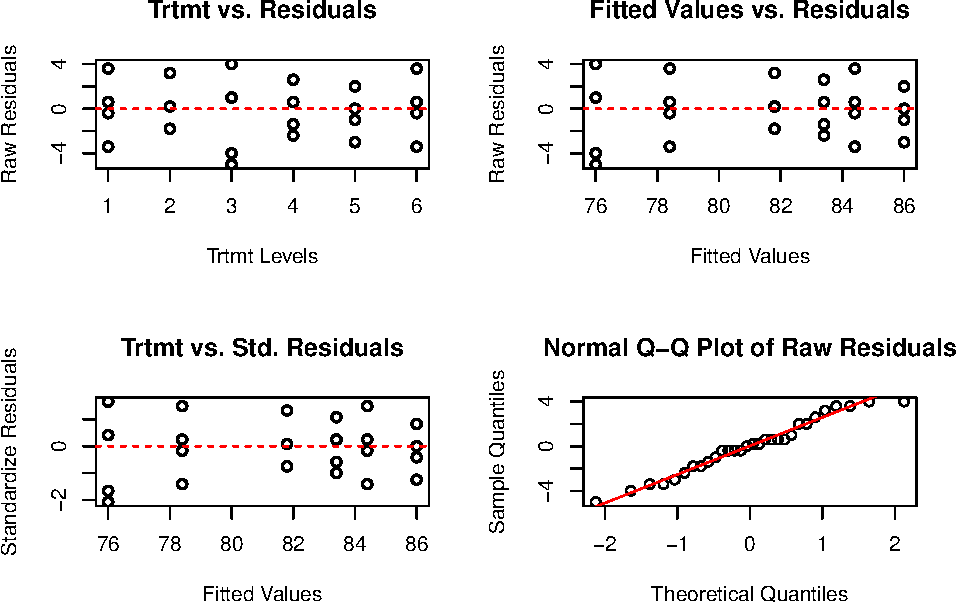
\includegraphics{Markdown_HW_5_files/figure-latex/unnamed-chunk-5-1.pdf}

Assuption (a): The error have mean 0:

Due to the formulation of the One Way ANOVA Model, the residuals always
sum up to 0.

Assuption (b): The error have constant variance:

By plotting the residuals against the fitted values of hte treatment
levels we saw no big difference in the pattern of the spread within the
groups. So we feel comfortable that the equal variance assumption is
approximately satisfied.

Since the the samples sizes of each group is equal, we can see that the
the expected result is strengthens the assumption.

Assuption (c): The error are nrmally distributed:

From the qq-plot above we see that the data is fairly straight and no
outliers are apparent. Therefore the normality assumption is reasonable.

Assuption (d): The error are independent:

Since we do not have any information on the

\subsection{Problem 2}\label{problem-2}

The spaghetti sauce experiment was run to compare the thicknesses of
three particular brands of spaghetti sauce, both when stirred and
unstirred. The six treatments were:

\begin{center}
1 = store brand, unstirred 2 = store brand, stirred\\
3 = national brand, unstirred 4 = national brand, stirred \\ 
5=gourmet brand,unstirred 6=gourmet brand,stirred
\end{center}

Part of the data collected is shown in Table 5.22. There are three
observations per treatment, and the response variable is the weight (in
grams) of sauce that flowed through a colander in a given period of
time. A thicker sauce would give rise to smaller weights.

\begin{enumerate}
\def\labelenumi{(\alph{enumi})}
\tightlist
\item
  Check the assumptions on the one-way analysis of variance model
  (3.3.1).
\end{enumerate}

\begin{Shaded}
\begin{Highlighting}[]
\NormalTok{spaghetti.sauce.data =}\StringTok{ }\KeywordTok{read.table}\NormalTok{(}\StringTok{"~/Desktop/Stats 6910/HW_4_and_5/spaghetti.sauce.txt"}\NormalTok{, }\DataTypeTok{header =} \OtherTok{TRUE}\NormalTok{)}

\NormalTok{spaghetti.sauce.data <-}\StringTok{ }\KeywordTok{as.data.frame}\NormalTok{(spaghetti.sauce.data)}
\NormalTok{spaghetti.sauce.data}\OperatorTok{$}\NormalTok{trtmt <-}\StringTok{ }\KeywordTok{as.factor}\NormalTok{(spaghetti.sauce.data}\OperatorTok{$}\NormalTok{trtmt)}


\NormalTok{spaghetti.model <-}\StringTok{ }\KeywordTok{aov}\NormalTok{(weight }\OperatorTok{~}\StringTok{ }\NormalTok{trtmt , }\DataTypeTok{data =}\NormalTok{ spaghetti.sauce.data)}
\KeywordTok{anova}\NormalTok{(spaghetti.model)}
\end{Highlighting}
\end{Shaded}

\begin{verbatim}
## Analysis of Variance Table
## 
## Response: weight
##           Df Sum Sq Mean Sq F value    Pr(>F)    
## trtmt      5 7976.4 1595.29  98.678 2.548e-09 ***
## Residuals 12  194.0   16.17                      
## ---
## Signif. codes:  0 '***' 0.001 '**' 0.01 '*' 0.05 '.' 0.1 ' ' 1
\end{verbatim}

\begin{Shaded}
\begin{Highlighting}[]
\CommentTok{# Get fitted values from the model}
\NormalTok{spaghetti.fitted <-}\StringTok{ }\KeywordTok{fitted}\NormalTok{(spaghetti.model); spaghetti.fitted}
\end{Highlighting}
\end{Shaded}

\begin{verbatim}
##        1        2        3        4        5        6        7        8 
## 17.00000 65.66667 23.00000 17.00000 23.00000 15.33333 58.00000 15.66667 
##        9       10       11       12       13       14       15       16 
## 15.66667 15.33333 58.00000 65.66667 23.00000 15.66667 17.00000 15.33333 
##       17       18 
## 65.66667 58.00000
\end{verbatim}

\begin{Shaded}
\begin{Highlighting}[]
\CommentTok{# Raw Residuals}
\NormalTok{spaghetti.raw.residuals <-}\StringTok{ }\KeywordTok{resid}\NormalTok{(spaghetti.model); spaghetti.raw.residuals}
\end{Highlighting}
\end{Shaded}

\begin{verbatim}
##             1             2             3             4             5 
## -3.000000e+00  3.333333e+00  3.000000e+00 -2.000000e+00 -3.000000e+00 
##             6             7             8             9            10 
## -3.333333e+00 -3.000000e+00 -1.666667e+00  3.333333e-01  6.666667e-01 
##            11            12            13            14            15 
##  8.000000e+00 -1.666667e+00 -6.217249e-15  1.333333e+00  5.000000e+00 
##            16            17            18 
##  2.666667e+00 -1.666667e+00 -5.000000e+00
\end{verbatim}

\begin{Shaded}
\begin{Highlighting}[]
\CommentTok{# Standardize residuals }
\NormalTok{spaghetti.stand.residuals <-}\StringTok{ }\KeywordTok{rstandard}\NormalTok{(spaghetti.model); spaghetti.stand.residuals }
\end{Highlighting}
\end{Shaded}

\begin{verbatim}
##          1          2          3          4          5          6 
## -0.9138115  1.0153462  0.9138115 -0.6092077 -0.9138115 -1.0153462 
##          7          8          9         10         11         12 
## -0.9138115 -0.5076731  0.1015346  0.2030692  2.4368308 -0.5076731 
##         13         14         15         16         17         18 
##  0.0000000  0.4061385  1.5230192  0.8122769 -0.5076731 -1.5230192
\end{verbatim}

\begin{Shaded}
\begin{Highlighting}[]
\KeywordTok{par}\NormalTok{(}\DataTypeTok{mfrow =} \KeywordTok{c}\NormalTok{(}\DecValTok{2}\NormalTok{,}\DecValTok{2}\NormalTok{))}
\CommentTok{#Raw Residuals vs. Frying/ Grilling fat content }
\KeywordTok{plot}\NormalTok{(}\KeywordTok{as.numeric}\NormalTok{(spaghetti.sauce.data}\OperatorTok{$}\NormalTok{trtmt) , spaghetti.raw.residuals, }
     \DataTypeTok{xlab =} \StringTok{"Codes"}\NormalTok{, }\DataTypeTok{ylab =} \StringTok{"Raw Residuals"}\NormalTok{, }\DataTypeTok{xaxt =} \StringTok{"n"}\NormalTok{,}
     \DataTypeTok{lwd =} \FloatTok{1.5}\NormalTok{)}
\KeywordTok{axis}\NormalTok{(}\DecValTok{1}\NormalTok{, }\DataTypeTok{at =} \DecValTok{1}\OperatorTok{:}\DecValTok{6}\NormalTok{, }\DataTypeTok{labels =} \KeywordTok{c}\NormalTok{(}\StringTok{"1"}\NormalTok{,}\StringTok{"2"}\NormalTok{,}\StringTok{"3"}\NormalTok{,}\StringTok{"4"}\NormalTok{,}\StringTok{"5"}\NormalTok{,}\StringTok{"6"}\NormalTok{))}
\KeywordTok{abline}\NormalTok{(}\DataTypeTok{h=}\DecValTok{0}\NormalTok{, }\DataTypeTok{col =} \StringTok{"red"}\NormalTok{, }\DataTypeTok{lty =} \DecValTok{2}\NormalTok{)}

\CommentTok{#Raw Residuals vs. Fitted Values}
\KeywordTok{plot}\NormalTok{(spaghetti.fitted , spaghetti.raw.residuals, }
     \DataTypeTok{xlab =} \StringTok{"Fitted Values"}\NormalTok{, }\DataTypeTok{ylab =} \StringTok{"Raw Residuals"}\NormalTok{,}
     \DataTypeTok{lwd =} \FloatTok{1.5}\NormalTok{)}
\KeywordTok{abline}\NormalTok{(}\DataTypeTok{h=}\DecValTok{0}\NormalTok{, }\DataTypeTok{col =} \StringTok{"red"}\NormalTok{, }\DataTypeTok{lty =} \DecValTok{2}\NormalTok{)}

\CommentTok{#Standardized Residuals vs. Fitted Values}
\KeywordTok{plot}\NormalTok{(spaghetti.fitted , spaghetti.stand.residuals, }
     \DataTypeTok{xlab =} \StringTok{"Fitted Values"}\NormalTok{, }\DataTypeTok{ylab =} \StringTok{"Standardize Residuals"}\NormalTok{,}
     \DataTypeTok{lwd =} \FloatTok{1.5}\NormalTok{)}
\KeywordTok{abline}\NormalTok{(}\DataTypeTok{h=}\DecValTok{0}\NormalTok{, }\DataTypeTok{col =} \StringTok{"red"}\NormalTok{, }\DataTypeTok{lty =} \DecValTok{2}\NormalTok{)}

\CommentTok{#Norma Probability Plot}
\KeywordTok{qqnorm}\NormalTok{(spaghetti.raw.residuals, }\DataTypeTok{main=} \StringTok{"Normal Q-Q Plot of Raw Residuals"}\NormalTok{)}
\KeywordTok{qqline}\NormalTok{(weights.raw.resid, }\DataTypeTok{col =} \StringTok{"red"}\NormalTok{)}
\end{Highlighting}
\end{Shaded}

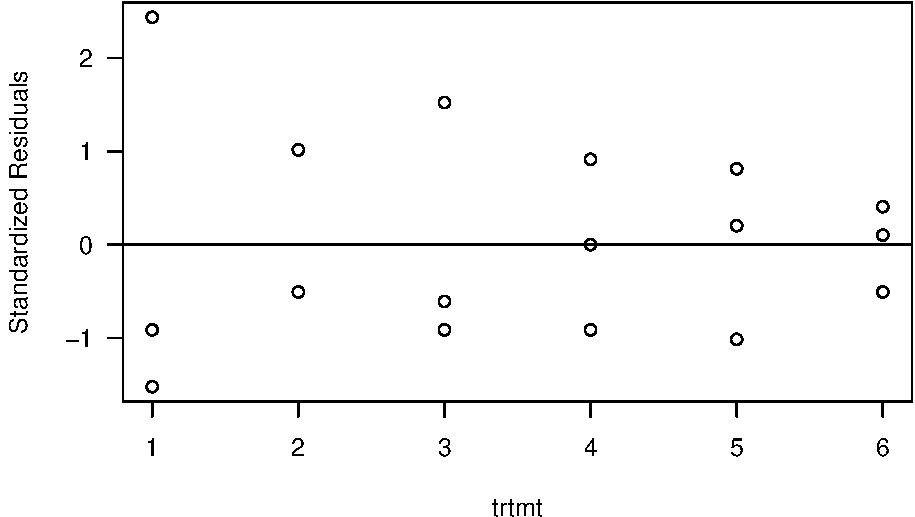
\includegraphics{Markdown_HW_5_files/figure-latex/unnamed-chunk-6-1.pdf}

\begin{enumerate}
\def\labelenumi{(\alph{enumi})}
\setcounter{enumi}{1}
\tightlist
\item
  Use Satterthwaite's method to obtain simultaneous confidence intervals
  for the six preplanned contrasts
\end{enumerate}

\[\tau_1 -\tau_2, \tau_3 -\tau_4, \tau_5 -\tau_6, \tau_1 -\tau_5, \tau_1 -\tau_3, \tau_3 -\tau_5,\]

Select an overall confidence level of at least 95\%.

We will use Tukey's since we want a simultaneous confidence intervals
for the six preplanned contrasts. Therefore,

A simultaius confidence interval for \(\tau_1 -\tau_2\) is
\((19.63595,-34.96928)\). A simultaius confidence interval for
\(\tau_3 -\tau_4\) is \((9.516045,-21.516045)\). A simultaius confidence
interval for \(\tau_5 -\tau_6\) is \((11.04009,-11.70676)\). A
simultaius confidence interval for \(\tau_1 -\tau_5\) is
\((69.58676,15.74657)\). A simultaius confidence interval for
\(\tau_1 -\tau_3\) is \((66.07661,15.92339)\). A simultaius confidence
interval for \(\tau_3 -\tau_5\) is \((17.18098,-13.84765)\).

The work is shown in the code below.

\begin{Shaded}
\begin{Highlighting}[]
\NormalTok{spaghetti.fitted}
\end{Highlighting}
\end{Shaded}

\begin{verbatim}
##        1        2        3        4        5        6        7        8 
## 17.00000 65.66667 23.00000 17.00000 23.00000 15.33333 58.00000 15.66667 
##        9       10       11       12       13       14       15       16 
## 15.66667 15.33333 58.00000 65.66667 23.00000 15.66667 17.00000 15.33333 
##       17       18 
## 65.66667 58.00000
\end{verbatim}

\begin{Shaded}
\begin{Highlighting}[]
\NormalTok{t_}\DecValTok{1}\NormalTok{ <-}\StringTok{ }\NormalTok{spaghetti.fitted[}\DecValTok{7}\NormalTok{]; t_}\DecValTok{1} \CommentTok{# tau_1}
\end{Highlighting}
\end{Shaded}

\begin{verbatim}
##  7 
## 58
\end{verbatim}

\begin{Shaded}
\begin{Highlighting}[]
\NormalTok{t_}\DecValTok{2}\NormalTok{ <-}\StringTok{ }\NormalTok{spaghetti.fitted[}\DecValTok{2}\NormalTok{];t_}\DecValTok{2} \CommentTok{# tau_2}
\end{Highlighting}
\end{Shaded}

\begin{verbatim}
##        2 
## 65.66667
\end{verbatim}

\begin{Shaded}
\begin{Highlighting}[]
\NormalTok{t_}\DecValTok{3}\NormalTok{ <-}\StringTok{ }\NormalTok{spaghetti.fitted[}\DecValTok{1}\NormalTok{]; t_}\DecValTok{3} \CommentTok{# tau_3}
\end{Highlighting}
\end{Shaded}

\begin{verbatim}
##  1 
## 17
\end{verbatim}

\begin{Shaded}
\begin{Highlighting}[]
\NormalTok{t_}\DecValTok{4}\NormalTok{ <-}\StringTok{ }\NormalTok{spaghetti.fitted[}\DecValTok{3}\NormalTok{];t_}\DecValTok{4}\CommentTok{# tau_4}
\end{Highlighting}
\end{Shaded}

\begin{verbatim}
##  3 
## 23
\end{verbatim}

\begin{Shaded}
\begin{Highlighting}[]
\NormalTok{t_}\DecValTok{5}\NormalTok{ <-}\StringTok{ }\NormalTok{spaghetti.fitted[}\DecValTok{6}\NormalTok{];t_}\DecValTok{5} \CommentTok{# tau_5}
\end{Highlighting}
\end{Shaded}

\begin{verbatim}
##        6 
## 15.33333
\end{verbatim}

\begin{Shaded}
\begin{Highlighting}[]
\NormalTok{t_}\DecValTok{6}\NormalTok{ <-}\StringTok{ }\NormalTok{spaghetti.fitted[}\DecValTok{8}\NormalTok{];t_}\DecValTok{6} \CommentTok{# tau_6}
\end{Highlighting}
\end{Shaded}

\begin{verbatim}
##        8 
## 15.66667
\end{verbatim}

\begin{Shaded}
\begin{Highlighting}[]
\CommentTok{#1st treatment variance}
\NormalTok{var_}\DecValTok{1}\NormalTok{ <-}\StringTok{ }\NormalTok{(}\KeywordTok{sd}\NormalTok{(spaghetti.sauce.data}\OperatorTok{$}\NormalTok{weight[spaghetti.sauce.data}\OperatorTok{$}\NormalTok{trtmt }\OperatorTok{==}\DecValTok{1}\NormalTok{]))}\OperatorTok{^}\DecValTok{2}\NormalTok{; var_}\DecValTok{1} 
\end{Highlighting}
\end{Shaded}

\begin{verbatim}
## [1] 49
\end{verbatim}

\begin{Shaded}
\begin{Highlighting}[]
\CommentTok{#2nd treatment variance}
\NormalTok{var_}\DecValTok{2}\NormalTok{ <-}\StringTok{ }\NormalTok{(}\KeywordTok{sd}\NormalTok{(spaghetti.sauce.data}\OperatorTok{$}\NormalTok{weight[spaghetti.sauce.data}\OperatorTok{$}\NormalTok{trtmt }\OperatorTok{==}\DecValTok{2}\NormalTok{]))}\OperatorTok{^}\DecValTok{2}\NormalTok{; var_}\DecValTok{2}
\end{Highlighting}
\end{Shaded}

\begin{verbatim}
## [1] 8.333333
\end{verbatim}

\begin{Shaded}
\begin{Highlighting}[]
\CommentTok{#3rd treatment variance}
\NormalTok{var_}\DecValTok{3}\NormalTok{ <-}\StringTok{ }\NormalTok{(}\KeywordTok{sd}\NormalTok{(spaghetti.sauce.data}\OperatorTok{$}\NormalTok{weight[spaghetti.sauce.data}\OperatorTok{$}\NormalTok{trtmt }\OperatorTok{==}\DecValTok{3}\NormalTok{]))}\OperatorTok{^}\DecValTok{2}\NormalTok{; var_}\DecValTok{3}
\end{Highlighting}
\end{Shaded}

\begin{verbatim}
## [1] 19
\end{verbatim}

\begin{Shaded}
\begin{Highlighting}[]
\CommentTok{#4th treatment variance}
\NormalTok{var_}\DecValTok{4}\NormalTok{ <-}\StringTok{ }\NormalTok{(}\KeywordTok{sd}\NormalTok{(spaghetti.sauce.data}\OperatorTok{$}\NormalTok{weight[spaghetti.sauce.data}\OperatorTok{$}\NormalTok{trtmt }\OperatorTok{==}\DecValTok{4}\NormalTok{]))}\OperatorTok{^}\DecValTok{2}\NormalTok{; var_}\DecValTok{4}
\end{Highlighting}
\end{Shaded}

\begin{verbatim}
## [1] 9
\end{verbatim}

\begin{Shaded}
\begin{Highlighting}[]
\CommentTok{#5th treatment variance}
\NormalTok{var_}\DecValTok{5}\NormalTok{ <-}\StringTok{ }\NormalTok{(}\KeywordTok{sd}\NormalTok{(spaghetti.sauce.data}\OperatorTok{$}\NormalTok{weight[spaghetti.sauce.data}\OperatorTok{$}\NormalTok{trtmt }\OperatorTok{==}\DecValTok{5}\NormalTok{]))}\OperatorTok{^}\DecValTok{2}\NormalTok{; var_}\DecValTok{5}
\end{Highlighting}
\end{Shaded}

\begin{verbatim}
## [1] 9.333333
\end{verbatim}

\begin{Shaded}
\begin{Highlighting}[]
\CommentTok{#6th treatment variance}
\NormalTok{var_}\DecValTok{6}\NormalTok{ <-}\StringTok{ }\NormalTok{(}\KeywordTok{sd}\NormalTok{(spaghetti.sauce.data}\OperatorTok{$}\NormalTok{weight[spaghetti.sauce.data}\OperatorTok{$}\NormalTok{trtmt }\OperatorTok{==}\DecValTok{6}\NormalTok{]))}\OperatorTok{^}\DecValTok{2}\NormalTok{; var_}\DecValTok{6}
\end{Highlighting}
\end{Shaded}

\begin{verbatim}
## [1] 2.333333
\end{verbatim}

\begin{Shaded}
\begin{Highlighting}[]
\CommentTok{# Confidence Interval for tau_i - tau_j}
\NormalTok{CI_Satterthwaite <-}\StringTok{ }\ControlFlowTok{function}\NormalTok{(t1,t2,variance_}\DecValTok{1}\NormalTok{,variance_}\DecValTok{2}\NormalTok{,r,v)\{}
 \CommentTok{#t1= 9.33; t2= 9.03;variance_1 = 2.95; variance_2 = 1.29; r= 10; v=4}
  
\CommentTok{# Numerator for Degree of Freedom}
\NormalTok{num_}\DecValTok{1}\NormalTok{ <-}\StringTok{ }\KeywordTok{sum}\NormalTok{(variance_}\DecValTok{1}\OperatorTok{/}\NormalTok{r,variance_}\DecValTok{2}\OperatorTok{/}\NormalTok{r)}\OperatorTok{^}\DecValTok{2}
\CommentTok{# Denominator for Degree of Freedom}
\NormalTok{den_}\DecValTok{1}\NormalTok{ <-}\StringTok{ }\KeywordTok{sum}\NormalTok{((variance_}\DecValTok{1}\OperatorTok{/}\NormalTok{r)}\OperatorTok{^}\DecValTok{2}\OperatorTok{/}\NormalTok{(r}\OperatorTok{-}\DecValTok{1}\NormalTok{), (variance_}\DecValTok{2}\OperatorTok{/}\NormalTok{r)}\OperatorTok{^}\DecValTok{2}\OperatorTok{/}\NormalTok{(r}\OperatorTok{-}\DecValTok{1}\NormalTok{))}
\CommentTok{#Degrees of freedom}
\NormalTok{deg.fr_tau1_tau2 <-}\StringTok{ }\NormalTok{num_}\DecValTok{1}\OperatorTok{/}\StringTok{ }\NormalTok{den_}\DecValTok{1}
\CommentTok{#Standard error}
\NormalTok{SE_}\DecValTok{1}\NormalTok{ <-}\StringTok{ }\KeywordTok{sqrt}\NormalTok{(}\KeywordTok{sum}\NormalTok{(variance_}\DecValTok{1}\OperatorTok{/}\NormalTok{r,variance_}\DecValTok{2}\OperatorTok{/}\NormalTok{r))}
\CommentTok{# w_T}
\NormalTok{w_}\DecValTok{1}\NormalTok{ <-}\StringTok{ }\KeywordTok{qtukey}\NormalTok{(.}\DecValTok{95}\NormalTok{,v,deg.fr_tau1_tau2)}\OperatorTok{/}\StringTok{ }\KeywordTok{sqrt}\NormalTok{(}\DecValTok{2}\NormalTok{)}
\CommentTok{# tau_i - tau_j}
\NormalTok{t1_min_t2 <-}\StringTok{ }\NormalTok{t1 }\OperatorTok{-}\StringTok{ }\NormalTok{t2}
\CommentTok{#return confidence interval}
\KeywordTok{return}\NormalTok{(CI_t1_min_t2 <-}\KeywordTok{c}\NormalTok{(t1_min_t2 }\OperatorTok{+}\StringTok{ }\NormalTok{w_}\DecValTok{1} \OperatorTok{*}\StringTok{ }\NormalTok{SE_}\DecValTok{1}\NormalTok{,t1_min_t2 }\OperatorTok{-}\StringTok{ }\NormalTok{w_}\DecValTok{1} \OperatorTok{*}\StringTok{ }\NormalTok{SE_}\DecValTok{1}\NormalTok{))}
\NormalTok{\}}


\NormalTok{CI_tau1_min_tau2 <-}\StringTok{ }\KeywordTok{CI_Satterthwaite}\NormalTok{(t_}\DecValTok{1}\NormalTok{,t_}\DecValTok{2}\NormalTok{,var_}\DecValTok{1}\NormalTok{,var_}\DecValTok{2}\NormalTok{,}\DecValTok{3}\NormalTok{,}\DecValTok{6}\NormalTok{);CI_tau1_min_tau2}
\end{Highlighting}
\end{Shaded}

\begin{verbatim}
##         7         7 
##  19.63595 -34.96928
\end{verbatim}

\begin{Shaded}
\begin{Highlighting}[]
\NormalTok{CI_tau3_min_tau4 <-}\StringTok{ }\KeywordTok{CI_Satterthwaite}\NormalTok{(t_}\DecValTok{3}\NormalTok{,t_}\DecValTok{4}\NormalTok{,var_}\DecValTok{3}\NormalTok{,var_}\DecValTok{4}\NormalTok{,}\DecValTok{3}\NormalTok{,}\DecValTok{6}\NormalTok{);CI_tau3_min_tau4 }
\end{Highlighting}
\end{Shaded}

\begin{verbatim}
##          1          1 
##   9.516045 -21.516045
\end{verbatim}

\begin{Shaded}
\begin{Highlighting}[]
\NormalTok{CI_tau5_min_tau6 <-}\StringTok{ }\KeywordTok{CI_Satterthwaite}\NormalTok{(t_}\DecValTok{5}\NormalTok{,t_}\DecValTok{6}\NormalTok{,var_}\DecValTok{5}\NormalTok{,var_}\DecValTok{6}\NormalTok{,}\DecValTok{3}\NormalTok{,}\DecValTok{6}\NormalTok{);CI_tau5_min_tau6}
\end{Highlighting}
\end{Shaded}

\begin{verbatim}
##         6         6 
##  11.04009 -11.70676
\end{verbatim}

\begin{Shaded}
\begin{Highlighting}[]
\NormalTok{CI_tau1_min_tau5 <-}\StringTok{ }\KeywordTok{CI_Satterthwaite}\NormalTok{(t_}\DecValTok{1}\NormalTok{,t_}\DecValTok{5}\NormalTok{,var_}\DecValTok{1}\NormalTok{,var_}\DecValTok{5}\NormalTok{,}\DecValTok{3}\NormalTok{,}\DecValTok{6}\NormalTok{);CI_tau1_min_tau5}
\end{Highlighting}
\end{Shaded}

\begin{verbatim}
##        7        7 
## 69.58676 15.74657
\end{verbatim}

\begin{Shaded}
\begin{Highlighting}[]
\NormalTok{CI_tau1_min_tau3 <-}\StringTok{ }\KeywordTok{CI_Satterthwaite}\NormalTok{(t_}\DecValTok{1}\NormalTok{,t_}\DecValTok{3}\NormalTok{,var_}\DecValTok{1}\NormalTok{,var_}\DecValTok{3}\NormalTok{,}\DecValTok{3}\NormalTok{,}\DecValTok{6}\NormalTok{);CI_tau1_min_tau3}
\end{Highlighting}
\end{Shaded}

\begin{verbatim}
##        7        7 
## 66.07661 15.92339
\end{verbatim}

\begin{Shaded}
\begin{Highlighting}[]
\NormalTok{CI_tau3_min_tau5 <-}\StringTok{ }\KeywordTok{CI_Satterthwaite}\NormalTok{(t_}\DecValTok{3}\NormalTok{,t_}\DecValTok{5}\NormalTok{,var_}\DecValTok{3}\NormalTok{,var_}\DecValTok{5}\NormalTok{,}\DecValTok{3}\NormalTok{,}\DecValTok{6}\NormalTok{);CI_tau3_min_tau5}
\end{Highlighting}
\end{Shaded}

\begin{verbatim}
##         1         1 
##  17.18098 -13.84765
\end{verbatim}


\end{document}
